\documentclass[11pt]{article}  % Use draft mode to speed up compilation

% First load extension packages
\usepackage[a4paper,margin=12.5mm]{geometry}    % page layout
\usepackage{setspace} \onehalfspacing         % line spacing
\usepackage{amsfonts,amssymb,amsmath}         % useful maths extensions
\usepackage{graphicx}                         % graphics import
\usepackage{siunitx}                          % easy SI units
\usepackage{cite}                             % better citations
\usepackage{hyperref}                         % hyperlinking
\usepackage{float}
\usepackage{adjustbox}
\usepackage{booktabs}
\usepackage{tabularx}
\usepackage{makecell}
\usepackage{tikz}
\usetikzlibrary{shapes.geometric, arrows.meta, positioning}
\newcolumntype{Y}{>{\raggedright\arraybackslash}X}
\newcolumntype{Z}{>{\raggedright\arraybackslash}X}

% Change paragraph indentation
\setlength{\parskip}{12pt}
\setlength{\parindent}{0pt}

% User-defined commands
\newcommand{\diff}[2]{\frac{\mathrm{d}{#1}}{\mathrm{d}{#2}}}
\newcommand{\ddiff}[2]{\frac{\mathrm{d}^2{#1}}{\mathrm{d}{#2}^2}}
\newcommand{\pdiff}[2]{\frac{\partial{#1}}{\partial{#2}}}
\newcommand{\pddiff}[2]{\frac{\partial^2{#1}}{\partial{#2}^2}}
\newcommand{\pdiffdiff}[3]{\frac{\partial^2{#1}}{\partial{#2}\partial{#3}}}
\renewcommand{\vec}[1]{\boldsymbol{#1}}
\newcommand{\Idx}{\;\mathrm{d}x}
\newcommand{\Real}{\mathbb{R}}
\newcommand{\Complex}{\mathbb{C}}
\newcommand{\Rational}{\mathbb{Q}}
\newcommand{\Integer}{\mathbb{Z}}
\newcommand{\Natural}{\mathbb{N}}

% topmatter
\title{Cognitive AI Coursework:  Integrating brain-inspired constraints in neural network models.}
\author{Dan Padian}
\date{\today}

% main body
\begin{document}
\maketitle

\tableofcontents
\newpage

%=============================================================================
% QUESTION 1: CRITICAL DISCUSSION (Max 4 pages total for a, b, c, d)
%=============================================================================
\section{Question 1: Brain-Inspired Constraints in Neural Networks}
\label{sec:question1}

% Critically discuss how changes to architecture, cost function, learning rule,
% and other factors can impose brain-like constraints on ANNs.
% Use equations and figures where helpful.
% Max 4 pages TOTAL for all subsections combined.

%-----------------------------------------------------------------------------
\subsection{Architecture [5 marks]}
\label{sec:q1_architecture}

Architectural modifications impose biologically grounded constraints by altering the structure and dynamics of artificial neural networks (ANNs). Whereas standard ANNs prioritise flexibility and ease of optimisation, biologically inspired architectures trade some of this flexibility to capture key organisational principles of real neural circuits.

Standard RNNs update their hidden state in discrete steps, which does not fully reflect the continuous, leaky integration of biological neurons. Leaky RNNs address this by introducing a membrane time constant $\tau$ that governs the rate at which activity decays relative to how much new input is incorporated:
\begin{equation}
\label{eq:leaky_rnn}
a(t) = a(t-1) + \frac{\Delta t}{\tau}\Big[-a(t-1) + f\big(W_{x \to a} x(t) + W_{a \to a} a(t-1) + b_1\big)\Big].
\end{equation}
The parameter $\tau$ therefore sets the effective temporal scale of each unit: smaller values produce fast, input-driven dynamics, whereas larger values enable slow, sustained integration. This mirrors functional differences observed in the brain, where sensory areas respond rapidly to changing inputs while higher-order regions integrate information over longer timescales for working memory and decision-making \cite{chaudhuri2015}.

A second biological principle is Dale's law, which states that a neuron is either exclusively excitatory or exclusively inhibitory across all its outputs \cite{Song2016}. This can be implemented by enforcing fixed weight signs after each update:
\begin{equation}
\label{eq:dales_law}
W^{\text{rec}} = W^{\text{rec},+} \odot D,
\end{equation}
where $W^{\text{rec},+}$ is the rectified recurrent weight matrix and $D$ is a diagonal matrix with $D_{ii}=+1$ for excitatory units and $D_{ii}=-1$ for inhibitory units. Typical cortical ratios (e.g., 80\% excitatory, 20\% inhibitory \cite{sahara2012fraction}) may be used or adjusted depending on the targeted brain region. Enforcing Dale’s law promotes excitatory--inhibitory balance and prevents units from arbitrarily switching signs, thereby encouraging stable recurrent computation through coordinated population dynamics.

Finally, biological neural circuits exhibit sparse connectivity: cortical neurons synapse onto only a small fraction of their potential targets (often as low as $\sim2\%$ in some areas or the brain \cite{lennie2003cost}). This can be simply modelled using binary masks:
\begin{equation}
W^{\text{rec}}_{\text{sparse}} = W^{\text{rec}}_{\text{dense}} \odot M,
\end{equation}
where $M_{ij} \in \{0,1\}$ specifies which connections are permitted. Sparse connectivity reduces the number of free parameters, improves interpretability by making information pathways explicit, and forces the network to develop structured representations under realistic wiring constraints.

In summary, these architectural modifications capture three core features of biological computation: temporal integration through membrane time constants, stable dynamics via excitatory--inhibitory balance, and structured information flow enabled by sparse anatomical connectivity.


% Discuss architectural constraints that make networks more brain-like:
% - Leaky integration / time constants
% - Dale's principle (E/I separation)
% - Sparse connectivity
% - Recurrent vs feedforward
% - Cell types and structured connectivity

% Examples:
% - Leaky RNN dynamics
% - E/I neuron separation
% - Sparse masks

% References: Song et al., 2016; Liu & Wang, 2024; course notes Week 4B

%-----------------------------------------------------------------------------
\subsection{Cost Function [5 marks]}
\label{sec:q1_cost}

The cost function is where biological constraints can be imposed most directly, as it dictates which network configurations are preferred during optimisation. By adding appropriate regularisation terms, learning can be steered towards operating to a state that can closely resemble those of biological neural circuits.

As noted in Section~\ref{sec:q1_architecture}, biological networks exhibit sparse connectivity \cite{lennie2003cost}, they can also have relatively low firing rates due to metabolic constraints \cite{amit1997dynamics}. These properties can be encouraged in artificial networks through regularisation penalties. First, L1 regularisation on synaptic weights promotes sparse connectivity:
\begin{equation}
\label{eq:l1_regularization}
J = J_{\text{task}} + \beta_{\text{L1,weight}} \sum_{i,j} |w_{i \to j}|.
\end{equation}
The absolute-value penalty pushes many weights toward zero, yielding connectivity matrices in which only essential links remain. Unlike fixed architectural masks (Section~\ref{sec:q1_architecture}), this approach allows the network to \emph{learn} which connections to prune, with $\beta_{\text{L1,weight}}$ controlling the sparsity--performance trade-off. However, it has no neuron distance plausibility as all connections are looked at equally.

Second, L2 regularisation on firing rates captures the metabolic cost of neural activity:
\begin{equation}
\label{eq:l2_regularization}
J = J_{\text{task}} + \beta_{\text{L2,rates}} \sum_{t=1}^{T} \sum_{i=1}^{N} a_{i,t}^2.
\end{equation}
Because activity is penalised quadratically, the network is encouraged to maintain low-amplitude firing while still supporting task-relevant dynamics. This tends to smooth hidden-state trajectories, prevent runaway excitation, and promotes stable recurrent computation.

Biological connectivity is also shaped by spatial structure: empirical studies show that connection probability decays exponentially with physical distance \cite{achterberg2023}. This can be modelled by embedding units in Euclidean space and penalising long-range connections:
\begin{equation}
J = J_{\text{task}} + \beta_{\text{WD}} \sum_{i,j} |w_{i \to j}| \times d_{i \to j},
\end{equation}
where $d_{i \to j}$ is the inter-unit distance. This encourages predominantly local wiring while permitting sparse long-range projections when functionally necessary, mirroring cortical organisation in which short-range connectivity dominates but strategic long-range links support inter-area communication.

Each regularisation term introduces trade-offs: excessively strong L1 penalties can prune connections essential for task performance, whereas weak penalties impose little biological structure ; large L2 penalties may suppress necessary transient responses and exacerbate vanishing gradients; and distance-based penalties depend sensitively on the chosen spatial embedding and decay profile. In practice, the $\beta$ hyperparameters must be tuned to balance biological realism against accuracy. Taken together, these cost-function terms provide complementary mechanisms for steering networks toward biologically plausible regimes by enforcing sparse wiring, low metabolic activity, and realistic spatial structure while remaining fully compatible with gradient-based optimisation.

\subsection{Learning Rule [5 marks]}
\label{sec:q1_learning}

The learning rule determines how synaptic weights change in response to activity and error signals, making it central to biological plausibility. Standard backpropagation suffers from three critical implausibilities: the weight transport problem (requiring $W = W^{\top}$), non-local credit assignment, and for recurrent networks, the \emph{perfect memory problem} which implies neurons must store and retrieve past activities with unrealistic precision. For temporal tasks, backpropagation through time (BPTT) exacerbates these issues by unrolling networks across dozens of timesteps, demanding that each unit perfectly recall its entire activity history.

Feedback alignment offers an effective way of addressing the weight-transport problem by replacing $W^{\top}$ with a fixed, randomly initialised feedback matrix $B$ \cite{lillicrap2016}.
\begin{equation}
\label{eq:feedback_alignment}
\Delta W \propto B \delta \quad \text{instead of} \quad W^{\top} \delta.
\end{equation}
During training, forward weights gradually align with random feedback pathways, allowing $B\delta$ to approximate true gradients without symmetric connectivity. However, this solves only the weight transport problem; the perfect memory issue remains for recurrent architectures.

For RNNs, Random Feedback Local Online (RFLO) learning provides a biologically plausible alternative to BPTT \cite{murray2019}. Rather than storing exact past activities, RFLO maintains a leaky co-activation trace:
\begin{equation}
p_{ab}(t) = \frac{1}{\tau}\phi'(u_a(t))h_b(t-1) + \left(1 - \frac{1}{\tau}\right)p_{ab}(t-1),
\end{equation}
where $\tau$ controls decay rate. Weight updates then combine random feedback with this trace: $\Delta W_{ab}(t) = \alpha [B\delta(t)]_a \times p_{ab}(t)$. Because traces decay naturally with the network's intrinsic timescale, RFLO eliminates both weight-transport and perfect-memory requirements while remaining “local” (updates depend only on information available at each synapse) and “online” (updates occur continuously during the forward pass, without storing full trajectories). 

Another approach is the dendritic error model, which exploits pyramidal neuron compartmentalisation \cite{sacramento2018}. Dendrites encode error signals ($\delta_2$) while somas maintain activity ($x_2$), yielding:
\begin{equation}
\frac{dW_1}{dt} = \alpha \left( g(x_2) - g(\delta_2) \right) x_1.
\end{equation}
This single-neuron implementation avoids weight transport, non-locality, and separate learning phases where all computations occur simultaneously within anatomically plausible structures.

Each approach trades off constraints: feedback alignment retains global error propagation but removes weight symmetry; RFLO sacrifices long-range temporal credit for local, online computation; dendritic models require specific cellular architecture. Together, they demonstrate that effective learning is possible under realistic biological constraints, though often with reduced capacity for complexity.

% Discuss biologically plausible learning rules:
% - Weight transport problem in backprop
% - Feedback alignment
% - RFLO (Random Feedback Local Online)
% - Hebbian learning
% - STDP (Spike-Timing-Dependent Plasticity)
% - Three-factor learning rules

% Key issue: Backprop uses W^T which is biologically unrealistic
% Solutions: Random feedback weights, local learning

% References: Lillicrap et al., 2016; Murray, 2019; Whittington & Bogacz, 2019

%-----------------------------------------------------------------------------
\subsection{Other Constraints [5 marks]}
\label{sec:q1_other}

Beyond architectural, cost-function, and learning rules, the learning construct itself imposes additional biological constraints. Three approaches (curriculum learning, three-factor learning rules, and reinforcement learning) capture principles of developmental progression, neuromodulatory control, and reward-driven adaptation that supervised backpropagation alone cannot model.


Biological learners acquire abilities gradually, mastering simpler behaviours before more complex ones. Curriculum learning formalises this by presenting training examples in an ordered progression starting from short, high signal-to-noise sequences to longer or noisier inputs as training stabilises. This staged exposure encourages robust representations, reduces early overfitting, and mirrors developmental trajectories in which sensory systems mature before higher-order cortical areas.

Hebbian plasticity is the technical name for the commonly known "cells that fire together, wire together" phrase. In the brain, plasticity is gated by neuromodulators such as dopamine and acetylcholine, which determine whether correlation leads to lasting modifications \cite{fremaux2016neuromodulated,kusmierz2017learning}. This can be implemented into an ANN as
\begin{equation}
\dot{w}_{ij} = y \cdot H(\text{pre}_i, \text{post}_j),
\end{equation}
where $y$ is a neuromodulatory signal and $H$ a Hebbian term. Only when $y>0$ does learning occur. Neuromodulatory gradients across cortex explain why some regions remain highly plastic \cite{froudist2023gradients}.


Supervised learning assumes explicit targets, which is a biologically implausible teaching signal as neurons do not receive detailed instructions about the correct firing pattern, nor a global error gradient to guide synaptic changes. Reinforcement learning replaces these with scalar rewards, directly paralleling dopaminergic reward prediction error (RPE) signals \cite{sutton2018reinforcement}. In temporal-difference learning,
\begin{equation}
V(s_t) \leftarrow V(s_t) + \alpha \big[r_{t+1} + \gamma V(s_{t+1}) - V(s_t)\big],
\end{equation}
the bracketed term corresponds to the RPE encoded by midbrain dopamine neurons. Q-learning extends this to action values:
\begin{equation}
Q(s_t,a_t) \leftarrow Q(s_t,a_t) + \alpha \big[r_{t+1} + \gamma \max_{a'} Q(s_{t+1},a') - Q(s_t,a_t)\big].
\end{equation}

A fundamental constraint in RL is the exploration-exploitation trade-off: agents must balance gathering information about uncertain options (explore) with maximising immediate rewards from known strategies (exploit). The $\varepsilon$-greedy policy implements this trade-off by selecting the highest-valued action with probability $1-\varepsilon$ (exploit) and a random action with probability $\varepsilon$ (explore) \cite{sutton2018reinforcement}. This mechanism mirrors biological decision-making, where dopaminergic modulation influences exploration. Higher dopamine levels increase exploratory behaviour, whilst lower levels promote exploitation of established policies. Decaying $\varepsilon$ schedules (e.g., from 1.0 to 0.1 over training) reflect developmental transitions from exploratory infancy to refined adult behaviour, capturing how biological learners shift from broad sampling to selective refinement as uncertainty decreases.

Deep RL methods such as DQN incorporate biologically inspired mechanisms including \emph{experience replay}, similar to hippocampal replay during sleep, and stochastic exploration policies reflecting behavioural variability. Model-based RL further aligns with hippocampal–prefrontal interactions supporting planning \cite{wang2018prefrontal}.


Together, these learning-paradigm constraints shape \emph{when}, \emph{how}, and \emph{from what signals} networks learn. Curriculum learning structures difficulty to support gradual skill acquisition; three-factor rules gate plasticity based on behavioural relevance; and reinforcement learning replaces omniscient supervision with sparse rewards that mirror dopaminergic teaching signals. These mechanisms complement earlier architectural and cost-function constraints by aligning training procedures with the temporal, modulatory, and reward-driven nature of biological learning.


%=============================================================================
% QUESTION 2: PRACTICAL IMPLEMENTATION
%=============================================================================
\newpage
\section{Question 2: NeuroGym Task Implementation}
\label{sec:question2}


\subsection{Question 2a: Model Implementation [10 marks / 3 pages]}
\label{sec:question2a}

\subsubsection{Task Selection: ReadySetGo}

The ReadySetGo task requires models to measure and reproduce temporal intervals, providing a direct assessment of their temporal processing capabilities, which are known to be fundamental to cognitive function \cite{chaudhuri2015}.

\begin{figure}[h]
    \centering
    \includegraphics[width=0.75\textwidth]{figures/readysetgo_task_structure.png}
    \caption{ReadySetGo task structure. Input stimuli showing Ready (yellow) and Set (green) cues for one trial, with fixation (blue) indicating when to initiate the response.}
    \label{fig:task_structure}
\end{figure}

As shown in Figure~\ref{fig:task_structure}, the model receives three inputs: Ready, Set, and fixation signals. The fixation input indicates when the model should produce its response, whilst the Ready and Set cues define the interval to be reproduced. The model must measure the Ready-to-Set interval ($t_s$) and reproduce it scaled by a gain factor of $g = 1.5$. This requires temporal integration over variable delays (500--2000\,ms), directly engaging the time constants and firing-rate regularisation discussed in Question~\ref{sec:q1_architecture}. The task mirrors interval timing processes in the prefrontal cortex, isolates temporal computation from working-memory demands, and remains computationally tractable whilst still sensitive to biological constraints \cite{remington2018flexible}.

\vspace{-0.3cm}
\subsubsection{Model Architectures}

To address this task, four models were defined, progressing from a minimal baseline to a biologically realistic architecture. Each model introduces additional constraints to the architecture, cost function, or learning rule.

\textbf{Model 1: Vanilla RNN (Baseline)}

A standard recurrent architecture with \texttt{tanh} activation, chosen for its bounded output range $[-1, 1]$, which prevents unstable activations whilst enabling both positive and negative firing rates. This model serves as the baseline against which biological constraints are evaluated.

\textbf{Model 2: Leaky RNN}

This model incorporates a membrane time constant of $\tau = 100$\,ms for temporal integration following Equation~\ref{eq:leaky_rnn}, implementing leaky dynamics where hidden-state decay is governed by $\tau$. Leaky integration supports sustained information retention across delays, which is essential for ReadySetGo's interval timing. Recurrent Gaussian noise ($\sigma_{\text{rec}} = 0.15$, $\xi_t \sim \mathcal{N}(0,1)$) reflects biological neural variability. The activation function is switched to ReLU to ensure non-negative firing rates, consistent with biological neurons.

\textbf{Model 3: Leaky RNN + Feedback Alignment}

Model~3 extends Model~2 by addressing the weight-transport problem through feedback alignment \cite{lillicrap2016}. The learning rule in Equation~\ref{eq:feedback_alignment} replaces the biologically implausible symmetric backward weights $W^\top$ with fixed random feedback weights $B$, such that $\Delta W \propto B\delta$. Forward propagation uses the trained weights $W$, whilst backpropagation employs the fixed matrix $B$, maintaining gradient-based optimisation without requiring symmetric connectivity. The matrix $B$ is initialised at the same scale as $W$ to prevent gradient explosion.

\textbf{Model 4: Biologically Realistic RNN}

Model~4 integrates four biological constraints: (1) feedback alignment (Equation~\ref{eq:feedback_alignment}); (2) Dale’s principle, enforcing an 80\% excitatory / 20\% inhibitory separation via Equation~\ref{eq:dales_law} whose ratio was chosen based on evidence seen in cortical circuits ~\cite{sahara2012fraction}; (3) L1 weight regularisation ($\beta_{L1}=10^{-5}$) from Equation~\ref{eq:l1_regularization}, promoting sparse connectivity; and (4) L2 firing-rate regularisation ($\beta_{L2}=0.01$) from Equation~\ref{eq:l2_regularization}, encouraging metabolically plausible activity levels. Together, these constraints combine learning, structural, and optimisation principles to assess how biological realism influences task performance.

\textbf{Progressive Architecture Design}

Figure~\ref{fig:model_progression} illustrates the stepwise introduction of biological constraints across the four architectures. This staged progression enables clean comparisons: starting from an unconstrained Vanilla baseline, each subsequent model adds one biological mechanism, isolating its specific effect on performance. The design directly tests the predictions in Question~1 about which constraints can be incorporated without degrading task competence. Comparing adjacent models highlights key trade-offs: Model~2 assesses the impact of temporal dynamics; Model~3 introduces a biologically plausible learning rule; and Model~4 evaluates whether a larger scale of biological realism remains compatible with effective supervised learning.


\begin{figure}[H]
\centering
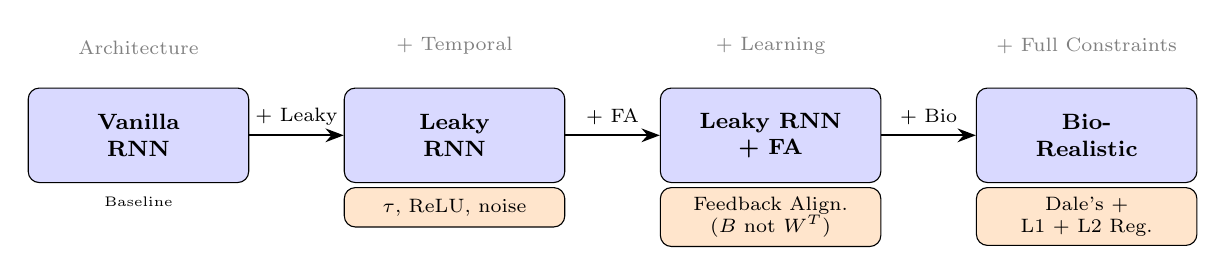
\begin{tikzpicture}[
    model/.style={rectangle, rounded corners, minimum width=2.8cm, minimum height=1.2cm,
                  text centered, draw=black, fill=blue!15, font=\bfseries\footnotesize, align=center},
    constraint/.style={rectangle, rounded corners, minimum width=2.8cm, minimum height=0.5cm,
                       text centered, draw=black, fill=orange!20, font=\scriptsize, align=center},
    arrow/.style={-Stealth, thick, black},
    label/.style={font=\tiny, align=center},
    node distance=0.3cm
]

\node (m1) [model] {Vanilla\\RNN};
\node (c1) [below=0.05cm of m1, label] {Baseline};

\node (arrow1) [right=1.2cm of m1] {};
\draw [arrow] (m1) -- node[above, font=\scriptsize] {+ Leaky} (arrow1);

\node (m2) [model, right=1.2cm of m1] {Leaky\\RNN};
\node (m2c) [constraint, below=0.05cm of m2] {$\tau$, ReLU, noise};

\node (arrow2) [right=1.2cm of m2] {};
\draw [arrow] (m2) -- node[above, font=\scriptsize] {+ FA} (arrow2);

\node (m3) [model, right=1.2cm of m2] {Leaky RNN\\+ FA};
\node (m3c) [constraint, below=0.05cm of m3] {Feedback Align.\\($B$ not $W^T$)};

\node (arrow3) [right=1.2cm of m3] {};
\draw [arrow] (m3) -- node[above, font=\scriptsize] {+ Bio} (arrow3);

\node (m4) [model, right=1.2cm of m3] {Bio-\\Realistic};
\node (m4c) [constraint, below=0.05cm of m4] {Dale's + \\L1 + L2 Reg.};

\node[above=0.3cm of m1, font=\scriptsize, text=gray] {Architecture};
\node[above=0.3cm of m2, font=\scriptsize, text=gray] {+ Temporal};
\node[above=0.3cm of m3, font=\scriptsize, text=gray] {+ Learning};
\node[above=0.3cm of m4, font=\scriptsize, text=gray] {+ Full Constraints};

\end{tikzpicture}
\caption{Progressive addition of biological constraints across the four model architectures. Purple boxes denote model types and beige boxes summarise the newly added constraints.}
\label{fig:model_progression}
\end{figure}

\subsubsection{Implementation Details}
\label{sec:implementation_models}

All models were trained for 4,000 steps using identical hyperparameters to ensure a fair comparison, as varying optimisation settings can obscure architectural effects. We used the Adam optimiser with a learning rate of $\alpha = 5 \times 10^{-4}$, chosen to balance convergence speed and stability particularly for biologically constrained models, where feedback alignment and sparsity penalties introduce gradient noise and make higher learning rates unstable. 

Each network employed 64 hidden units, a compromise between computational efficiency and representational capacity: smaller models struggled to encode long intervals, whereas larger ones offered no measurable benefit but increased training variance. The timestep $\Delta t = 20$\,ms similarly balances numerical accuracy against computational cost, remaining biologically plausible while keeping sequence lengths tractable. The leaky models have $\tau=100$ms which is a longer spike time typically than traditional neuron but allows a smaller 64 hidden neuron model to complete the task. 

Recurrent Gaussian noise ($\sigma_{\text{rec}} = 0.1$, $\xi_t \sim \mathcal{N}(0,1)$) was added only to the leaky-based models (Models~2--4) to approximate biological neural variability and avoid overly deterministic dynamics. Noise was omitted from the Vanilla RNN to preserve its role as a clean baseline.

The loss combined cross-entropy task loss with additional biological regularisation terms for Model~4. Class weights of $(0.1, 1.0)$ for fixation versus action outputs addressed the strong class imbalance in timing tasks: the model fixes for most of each trial and produces an action only at the reproduced interval. Without weighting, models tended to overpredict fixation, achieving low loss without learning the intended timing behaviour.

\vspace{-0.3cm}
\subsubsection{Learning Performance}
\vspace{-0.2cm}

As shown in Figure~\ref{fig:learning_curves}, all models converged successfully, achieving task loss below 0.20, indicating that biological constraints remain broadly compatible with effective temporal learning. Although early learning rates were comparable, their trajectories diverged. The Vanilla RNN plateaued around 0.17, while the Leaky~+~FA model showed a similar slowdown, consistent with the reduced precision introduced by random feedback weights.

In contrast, the Leaky RNN achieved the strongest overall performance, continuing to improve throughout training and reaching a final task loss of approximately 0.10, with signs of further potential improvement. This suggests that leaky integration provides a strong inductive bias for interval timing, consistent with theories that slow membrane dynamics naturally support temporal processing even without additional biological structure \cite{paton2018neural} (uses its own decay to keep track of time). The Bio-realistic model exhibited particularly interesting behaviour: after a prolonged plateau near step~1000, it underwent a rapid drop in loss, falling to approximately 0.14 within only 250 steps. This “clicking” dynamic suggests that the combination of feedback alignment and activity regularisation can stabilise training sufficiently for FA to become effective rather than detrimental.

\vspace{-0.2cm}
\begin{figure}[H]
    \centering
    \includegraphics[width=0.75\textwidth]{figures/question_2a_results.png}
    \caption{Learning curves showing task loss only, for fair comparison across models. All architectures successfully learn the timing task to different levels.}
    \label{fig:learning_curves}
\end{figure}



\newpage
\subsection{Question 2b: Hidden Unit Activity Analysis [20 marks / 4 pages]}
\label{sec:question2b}

\subsubsection{Performance Comparison}

Despite similar training losses ($\approx 0.20$), Figure~\ref{fig:timing_performance} reveals dramatic performance differences. Vanilla RNN exhibits linear scaling but systematic undershooting due to an incompletely learnt offset bias. In contrast, Leaky RNN and Bio-Realistic achieve near-perfect performance (Leaky: $\mu=-70$ms, $\sigma=35$ms; Bio-Realistic: $\mu=-23$ms, $\sigma=24$ms), demonstrating that leaky integration and sparsity constraints do not impair temporal precision. Leaky+FA, however, shows severe underprediction ($\mu=-440$ms, $\sigma=230$ms), confirming that feedback alignment impairs temporal credit assignment when rewards are delayed unless compensated by additional regularisation. Vanilla's timing variability ($\sigma=250$ms) falls within biological ranges observed in reaction time tasks, suggesting moderate biological plausibility despite lacking explicit constraints. 


\begin{figure}[H]
    \centering
    \includegraphics[width=0.9\textwidth]{figures/readysetgo_timing.png}
    \caption{Timing performance analysis across models. \textbf{Left:} Scatter plot showing target versus produced intervals, with black diagonal indicating perfect timing. Leaky RNN (orange) and Bio-Realistic (red) clusters near-perfectly along the diagonal, whilst Leaky+FA (green) and vanilla (blue) systematically undershoot. \textbf{Right:} Error distributions with mean ($\mu$) and standard deviation ($\sigma$) revealing systematic biases and precision differences. Fixed 50ms bin width enables direct comparison across models.}
\label{fig:timing_performance}
\end{figure}

\subsubsection{Neural Population Dynamics}

PCA trajectories (Fig.~\ref{fig:trajectories}) reveal distinct computational strategies shaped by architectural constraints. Vanilla RNN exhibits highly compressed dynamics (PC1: 93.4\%), suggesting fixed attractor dynamics unable to flexibly encode multiple intervals. Trajectories collapse onto a single path regardless of interval duration. Leaky RNN displays 10 parallel trajectories (PC1: 63.9\%), where different intervals occupy separate manifold paths, resembling primate prefrontal dynamics during interval timing \cite{remington2018flexible}. Leaky+FA shows similar parallel structure but higher compression (PC1: 94\%), indicating that feedback alignment regularises representations to lower dimensionality, thereby reducing interval discriminability and explaining the systematic timing bias. Bio-Realistic exhibits moderately compressed trajectories (PC1: 83.3\%) with sparse, intermittent activity mirroring biological recordings; high PC1 variance reflects sparsity rather than genuine low dimensionality.

Critically, across all models, Ready and Go cues occupy consistent state-space regions whilst Set positions vary systematically with interval duration. This geometric encoding implements a clock mechanism where manifold position directly represents elapsed time. Neurons are set ready, then traverse a loop proportional to the delay duration before producing the go signal. This pattern is particularly evident in Leaky RNN and Bio-Realistic architectures.

\begin{figure}[H]
    \centering
    \includegraphics[width=0.9\textwidth]{figures/readysetgo_trajectories.png}
    \caption{Neural trajectories in PCA space (10 trials per model). Green circles mark Ready (trial start), blue diamonds mark Set (cue), red squares mark Go (response).}
    \label{fig:trajectories}
\end{figure}

\subsubsection{Neural Activity Patterns and Functional Specialisation}

Activity heatmaps (Fig.~\ref{fig:heatmaps}) reveal distinct sparsity gradients and specialisation strategies across architectures. Vanilla exhibits dense sustained firing ($\sim$45 active neurons) with binary activity patterns showing a distributed coding strategy lacking temporal precision. Leaky RNN maintains dense activity but with structured temporal bursts during interval encoding. Both Leaky+FA and Bio-Realistic activate only $\sim$20 neurons concentrated around the Set cue, with the top 10 neurons dominating. This forms the previously spoken about specialised "timing circuit" that is metabolically efficient but potentially fragile due to reliance on few critical units.

Individual neuron activity reveals key patterns. Leaky RNN neurons 15--30 exhibit firing rates that increase linearly with slopes proportional to the sample interval duration. This confirms that leaky integration ($\tau=100$ms) implements temporal accumulation rather than discrete state transitions. Vanilla shows weak ramping with abrupt state transitions, explaining its systematic under-prediction. Bio-Realistic exhibits irregular, noisy ramping reflecting stochastic sparse recruitment. Across models, ramping neurons maintain elevated activity until Go (working memory function), whilst separate units show transient Set/Go bursts (readout function). 

\begin{figure}[!h]
    \centering
    \includegraphics[width=0.75\textwidth]{figures/readysetgo_heatmaps.png}
    \caption{Activity heatmaps showing 64 neurons over time for a single trial across models. Cyan dashed line marks Set cue, lime dashed line marks expected Go response. Vertical axis: neuron index, horizontal axis: time, colour: activity magnitude. }
    \label{fig:heatmaps}
\end{figure}

\begin{figure}[!h]
    \centering
    \includegraphics[width=0.75\textwidth]{figures/readysetgo_connectivity.png}
    \caption{Recurrent connectivity matrices for ReadySetGo models. Red/blue colourmap shows excitatory/inhibitory connection strengths. Bio-Realistic model (bottom-right) exhibits structured excitatory-inhibitory organisation, while other models show dense mixed connectivity. Sparsity statistics indicate the proportion of near-zero weights in each architecture.}
    \label{fig:readysetgo_connectivity}
\end{figure}


Figure~\ref{fig:readysetgo_connectivity} visualises recurrent connectivity patterns across models. A striking transition occurs from Leaky+FA to Bio-Realistic: sparsity increases dramatically from 7.28\% to 79.7\% due to L1 regularisation, accompanied by a sixfold decrease in average connection strength. The Bio-Realistic matrix exhibits clear structure imposed by Dale's law seen on the right-hand side showing the excitatory-inhibitory boundary, reflecting that Dale's principle constrains neuronal output rather than input connectivity. This 79.7\% sparsity approaches biologically observed cortical values ($\sim$98\% \cite{lennie2003cost}), yet the network achieves superior timing performance, demonstrating that structured sparse connectivity can enhance rather than impair function when appropriately regularised. This sparsity level appears near-optimal: further increases degraded task loss during extra experiments, suggesting a critical threshold balancing metabolic efficiency against computational capacity.

\subsubsection{Computational Mechanisms for Interval Timing}

These analyses reveal how architectural constraints shape task solutions. Successful models (Leaky RNN, Bio-Realistic) solve the timing task through ramping integration. Neurons accumulate activity linearly during Ready→Set such that peak firing rate encodes interval duration $t_s$. Recurrent dynamics then maintain this information in working memory until reproduction. The geometric encoding (Fig.~\ref{fig:trajectories}) implements this spatially. The network state traverses paths whose length represents elapsed time, with different intervals occupying parallel trajectories that enable unambiguous differences. Leaky integration's $\tau=100$ms time constant enables this sustained accumulation, preventing the rapid decay that causes Vanilla's weak ramping and systematic underprediction. Conversely, feedback alignment compresses representations to lower dimensionality (PC1: 94\%) to reduce sensitivity to noisy gradients. This degrades interval decipherability. Trajectories remain parallel but closer in state space, causing errors and timing bias. Bio-Realistic's success despite extreme sparsity (79.7\%) reflects structured specialisation: L1 regularisation creates a dedicated timing circuit ($\sim$15 neurons) implementing ramping integration, whilst Dale's law stabilises this sparse population through excitatory-inhibitory balance, demonstrating that biological constraints enhance performance when imposed jointly rather than in isolation.

\subsubsection{Summary of Findings}

Trained models reveal distinct computational strategies shaped by biological constraints. Leaky RNN and Bio-Realistic achieve near-optimal timing performance ($\mu \approx -50$ms, $\sigma \approx 30$ms) through complementary mechanisms: Leaky RNN used parallel manifold trajectories with moderate neuronal use ($\sim$30 neurons), whilst Bio-Realistic uses extreme sparsity ($\sim$15 neurons, 79.7\% sparse connectivity) approaching biological levels. Both successfully implement linear ramping dynamics for temporal accumulation. In contrast, Vanilla and Leaky+FA exhibit systematic offset biases ($\mu < -250$ms) despite achieving low training loss. Vanilla shows this due to weak ramping and compressed dynamics. Leaky+FA shows this due to feedback alignment's dimensionality reduction.

Critically, all models converge on geometric temporal encoding: Set cue positions vary systematically along manifolds whilst Ready and Go occupy consistent regions, implementing clocks where state-space location represents elapsed time. This convergent solution suggests geometric encoding is fundamental to interval timing regardless of architectural constraints. These findings demonstrate that biological constraints such as Dale's law, sparse connectivity, and feedback alignment remain compatible with effective temporal learning but introduce specific trade-offs. Sparsity enhances metabolic efficiency without impairing performance when combined with appropriate regularisation. Feedback alignment compresses representational dimensionality, causing systematic biases unless counterbalanced by additional constraints.

%-----------------------------------------------------------------------------
% QUESTION 2C: SECOND TASK (Max 4 pages)
%-----------------------------------------------------------------------------

\newpage

\subsection{Question 2c: Second Task Analysis [20 marks / 4 pages]}
\label{sec:question2c}

To assess whether biological constraints are task-general or task-specific, the four architectures are evaluated on \texttt{MultiSensoryIntegration-v0}, a perceptual decision-making task requiring probabilistic evidence accumulation. This contrasts with ReadySetGo's sustained temporal integration ($\tau=100$ms), testing whether Section~\ref{sec:question2b}'s findings generalise.

\subsubsection{Task Description}

\texttt{MultiSensoryIntegration-v0} presents two simultaneous sensory streams (modality 1 and 2), each with left/right channels. Figure~\ref{fig:q2_multisensory_task_structure} shows five input streams: fixation (row 1), mod1-left/right (rows 2--3), mod2-left/right (rows 4--5). Trial difficulty depends on (i) \textbf{coherence}-evidence strength, and (ii) \textbf{weight}-reliability assigned to modality 1 versus 2. The agent fixates during stimuli, integrates both modalities weighted by reliability, then emits a binary left/right decision.

\begin{figure}[H]
    \centering
    \includegraphics[width=0.75\textwidth]{figures/q2_multisensory_task_structure.png}
    \caption{Task structure: three trials showing fixation (row 1), modality 1/2 left/right channels (rows 2--5), and decision output (top: green=left, red=right).}
    \label{fig:q2_multisensory_task_structure}
\end{figure}

\vspace{-0.3cm}
Unlike ReadySetGo's sustained integration over variable delays (500--2000ms), this requires snapshot evidence accumulation of brief stimulus periods ($\sim$200--500ms) without maintaining interval representations in working memory. This tests whether Section~\ref{sec:question2b}'s mechanisms (ramping integration, geometric encoding, sparse circuits) generalise or reflect task-specific adaptations.

\subsubsection{Training and Performance}

All architectures were trained identically to ReadySetGo (supervised learning, cross-entropy loss, Adam optimiser, matching hyperparameters). Training loss decays smoothly, stabilising by $\sim$8,000 steps (Fig.~\ref{fig:q2_multisensory_training_curves}). Unlike ReadySetGo where Bio-Realistic showed delayed convergence (step 1000 "clicking"), all models converge similarly here, suggesting biological constraints affect sustained temporal integration more than snapshot accumulation.

\begin{figure}[H]
    \centering
    \includegraphics[width=0.75\textwidth]{figures/q2_multisensory_training_curves.png}
    \caption{Training loss (log scale) for all architectures; y-lim fixed to 0.05–0.20.}
    \label{fig:q2_multisensory_training_curves}
\end{figure}


%5\begin{table}[h!]
%centering
%\small
%\setlength{\tabcolsep}{12pt}
%\begin{tabular}{c c c c}
%\hline
%\textbf{Vanilla RNN} & \textbf{Leaky RNN} & %\textbf{Leaky + FA} & \textbf{Bio-%realistic} \\
%\hline
%0.926 & 0.904 & 0.898 & 0.898 \\
%\hline
%\end{tabular}
%\end{table}




\begin{table}[H]
\centering
\small
\caption{Confusion matrices for Left vs Right decision performance across all four models. Each 2x2 matrix shows predicted vs ground truth classifications for decision trials only (fixation trials excluded).}
\label{fig:q2_multisensory_confusion_matrices}
\setlength{\tabcolsep}{20pt}
\renewcommand{\arraystretch}{1.3}

\begin{tabular}{c c c c}

\makecell{\textbf{Vanilla RNN}\\(Acc = 0.906)} &
\makecell{\textbf{Leaky RNN}\\(Acc = 0.910)} &
\makecell{\textbf{Leaky + FA}\\(Acc = 0.896)} &
\makecell{\textbf{Bio-realistic}\\(Acc = 0.918)} \\[4pt]

$\begin{pmatrix}
231 & 32 \\
15 & 222
\end{pmatrix}$
&
$\begin{pmatrix}
247 & 12 \\
33 & 208
\end{pmatrix}$
&
$\begin{pmatrix}
244 & 14 \\
38 & 204
\end{pmatrix}$
&
$\begin{pmatrix}
224 & 13 \\
28 & 235
\end{pmatrix}$

\end{tabular}
\end{table}


\vspace{-0.3cm}
All models achieve high accuracy ($>89\%$, Table~\ref{fig:q2_multisensory_confusion_matrices}), contrasting sharply with ReadySetGo's variable timing precision ($\mu$: $-23$ms to $-440$ms). Strikingly, Leaky+FA's severe timing bias ($\mu=-440$ms) vanishes (91.0\% accuracy, no bias), revealing feedback alignment's dimensionality compression impairs \emph{temporal} credit assignment where continuous intervals require high-dimensional manifolds, but handles categorical decisions effectively. This validates Question 1's prediction of domain-specific learning limitations. Bio-Realistic achieves highest accuracy (91.8\%), demonstrating extreme sparsity and E/I balance enhance categorical performance, contrasting with timing where they matched but did not exceed Leaky RNN.

\subsubsection{Hidden Unit Analysis}

PCA (Fig.~\ref{fig:q2_multisensory_pca}) reveals dramatically different geometry than ReadySetGo. Timing required parallel trajectories encoding continuous intervals (Leaky RNN PC1: 63.9\%, 10 paths); integration compresses to binary left/right clusters in 2D (Vanilla PC1--2: $\sim$95\%). This reflects computational demands: timing needs high-dimensional manifolds where trajectory \emph{position} encodes elapsed time geometrically; categorical decisions collapse evidence onto a single axis with no temporal history needed, only final accumulated evidence. Bio-Realistic achieves high PC1 variance in both tasks (ReadySetGo: 83.3\%, Integration: $\sim$90\%), confirming sparsity and E/I balance universally reduce dimensionality regardless of task structure. 

\begin{figure}[!h]
    \centering
    \includegraphics[width=0.75\textwidth]{figures/q2_multisensory_pca.png}
    \caption{PCA of per-trial mean hidden states (rows = models, colored by decision).}
    \label{fig:q2_multisensory_pca}
\end{figure}


\begin{figure}[!h]
    \centering
    \includegraphics[width=0.75\textwidth]{figures/q2_multisensory_heatmaps.png}
    \caption{Hidden-unit activity heatmaps (correct trials, averaged) for all models.}
    \label{fig:q2_multisensory_heatmaps}
\end{figure}

\begin{figure}[!h]
    \centering
    \includegraphics[width=0.75\textwidth]{figures/q2_multisensory_connectivity.png}
    \caption{Recurrent connectivity matrices showing weight structure across models. Red indicates positive (excitatory) weights, blue indicates negative (inhibitory) weights.}
    \label{fig:q2_multisensory_connectivity}
\end{figure}

Heatmaps (Fig.~\ref{fig:q2_multisensory_heatmaps}) confirm task-invariant sparsity: Bio-Realistic uses $\sim$25--30 neurons (matching timing's $\sim$15--20), whilst Vanilla/Leaky activate broadly ($\sim$40--45) across both tasks, validating L1/L2 regularisation universally enforces metabolic efficiency. However, temporal dynamics differ: ReadySetGo showed sustained ramping (linear accumulation encoding $t_s$); integration exhibits brief transient bursts where networks accumulate evidence rapidly then maintain the decision variable. 

Connectivity (Fig.~\ref{fig:q2_multisensory_connectivity}) shows Bio-Realistic reaches 91\% sparsity versus 79.7\% in ReadySetGo, approaching biological cortical values ($\sim$98\% \cite{lennie2003cost}). Higher sparsity suggests categorical tasks permit more aggressive pruning where binary decisions need fewer connections than continuous interval encoding. Dale's law imposes similar E/I structure (blue inhibitory weights, right) across tasks, confirming excitatory-inhibitory balance is task-general, though specific connectivity patterns adapt to computational requirements. 

\subsubsection{Summary and Cross-Task Insights}

Cross-task comparison directly tests Section~\ref{sec:question2b}'s predictions, revealing which biological constraints are task-general versus task-specific. Architectural constraints prove task-general: sparsity (L1/L2) and E/I balance (Dale's law) enforce consistent dimensionality reduction, metabolic efficiency ($\sim$15--30 neurons), and sparse connectivity (79--91\%) across both tasks, validating Question 1's cost-function principles. Bio-Realistic achieves highest integration accuracy (91.8\%) whilst matching timing performance ($\mu=-23$ms), demonstrating biological constraints can enhance categorical decisions without impairing temporal integration. Conversely, learning rules exhibit task-specific effects: feedback alignment's catastrophic timing bias ($\mu=-440$ms) vanishes in integration (91.0\%), confirming FA's dimensionality compression (PC1: 94\%) impairs continuous interval discrimination but handles binary categorical decisions effectively. Leaky integration's $\tau=100$ms proves critical for timing but dispensable for integration, explaining why Vanilla matches Leaky here (90.6\% vs 91.0\%) but fails dramatically on timing ($\mu=-324$ms). These findings demonstrate biological plausibility can be completely compatible with diverse cognitive tasks through modular design.

\newpage


\subsection{Question 2d: Original Contribution - Model-Free Reinforcement Learning}
\label{sec:question2d}

Supervised learning, whilst effective in Sections~\ref{sec:question2a}--\ref{sec:question2c}, is biologically implausible as natural environments provide scalar reward signals, not explicit per-timestep targets. Sections~\ref{sec:question2b} and~\ref{sec:question2c} demonstrated that architectures achieving high supervised accuracy (Leaky RNN, Bio-Realistic: $\sim$90--92\%) exploit dense gradient signals to overcome biological constraints, whilst feedback alignment's limitations emerge only in specific contexts (timing bias: $\mu=-440$ms). Reinforcement learning (RL) formalises reward-driven learning via dopaminergic reward prediction errors \cite{schultz1997neural}, offering a neurobiologically realistic framework testing whether biological constraints viable under dense supervision remain effective with sparse feedback. This section evaluates whether the four architectures can learn \texttt{MultiSensoryIntegration-v0} via Deep Q-Networks (DQN), incorporating hippocampal experience replay to test whether supervised performance (91\% accuracy) translates to sparse reward scenarios.

\subsubsection{Q-Learning and Biological Plausibility}

Q-learning \cite{watkins1989} learns action-value functions $Q(s,a)$ representing the expected cumulative reward for taking action $a$ in state $s$. The update rule follows temporal-difference learning:
\begin{equation}
Q(s_t, a_t) \leftarrow Q(s_t, a_t) + \alpha \big[r_{t+1} + \gamma \max_{a'} Q(s_{t+1}, a') - Q(s_t, a_t)\big],
\end{equation}
where $\alpha$ is the learning rate, $\gamma$ the discount factor, and the bracketed term is the reward prediction error (RPE). This RPE mirrors dopamine neuron activity in midbrain structures: dopamine firing increases when rewards exceed predictions ($r_{t+1} > Q(s_t,a_t)$) and decreases when rewards fall short, precisely matching the TD error signal observed in biological circuits \cite{schultz1997neural}.

This implementation is \emph{model-free}: it learns values directly from experience without building an explicit environment model, contrasting with model-based methods (e.g., Dyna-Q) that construct cognitive maps for planning \cite{tolman1948}. Action selection follows an $\varepsilon$-greedy policy: with probability $1-\varepsilon$, the agent exploits $\arg\max_a Q(s,a)$; with probability $\varepsilon$, it explores uniformly. Unlike supervised learning's dense per-timestep targets, RL uses only sparse scalar rewards, making optimisation slower and amplifying architectural weaknesses. Feedback alignment struggles with delayed credit assignment, whilst Bio-Realistic sparsity creates fragile dependencies that exploration may never discover.


\subsubsection{Implementation Details}

The DQN agent was trained on \texttt{MultiSensoryIntegration-v0} using the four architectures from Section~\ref{sec:question2a}, maintaining identical hyperparameters for fair comparison: 64 hidden units, $\tau=100$ms, $\sigma_{\text{rec}}=0.15$, learning rate $\alpha=5 \times 10^{-4}$. Bio-Realistic models retained L1 weight regularisation ($\beta_{L1}=5 \times 10^{-4}$) and L2 firing rate regularisation ($\beta_{L2}=0.01$). Training proceeded for 5,000 episodes with batch size 16. Table~\ref{tab:implementation_of_dqn} provides a holistic overview of the RL framework.

\begin{table}[!h]
\centering
\small
\caption{RL implementation components for DQN training on \texttt{MultiSensoryIntegration-v0}.}
\label{tab:implementation_of_dqn}
\renewcommand{\arraystretch}{1.2}
\setlength{\tabcolsep}{6pt}
\begin{tabular}{p{0.18\textwidth} p{0.80\textwidth}}
\textbf{Component} & \textbf{Description} \\ \hline

\textbf{Agent} &
RNN processing observation sequences, outputting Q-values $Q(s,a;\theta)$ for actions \{fixate, left, right\}. \\

\textbf{Environment} &
\texttt{MultiSensoryIntegration-v0} task (5 input channels: fixation + 4 sensory modalities). \\

\textbf{Reward Signal} &
Scalar reward: $+1$ for correct choice, $-5$ for incorrect choice or fixation termination, $0$ otherwise. Strong penalties prevent degenerate fixation-only policies. \\

\textbf{Value Function} &
Q-network approximates $Q(s,a)$; separate target network stabilises bootstrapped TD targets. \\

\textbf{Policy} &
$\varepsilon$-greedy with linear decay from $\varepsilon=1.0 \to 0.15$ over 80\% of training episodes. \\

\textbf{Experience Replay} &
Buffer capacity 10,000 transitions; random sampling (batch size 16) breaks temporal correlations, mirroring hippocampal replay. \\

\end{tabular}
\end{table}


Critically, the RNN maintains full observation history at each timestep, forming sequences of shape $[T, \text{batch}, \text{obs\_dim}]$. Q-values from the \emph{final} timestep determine action selection, enabling temporal integration across fixation and stimulus periods before decisions. This mirrors how prefrontal circuits accumulate evidence over time before committing to a choice.

\subsubsection{Results and Analysis}

\begin{figure}[!h]
    \centering
    \includegraphics[width=0.75\textwidth]{figures/question_2d_MSI_dqn_rewards.png}
    \caption{Reward curves for DQN training on \texttt{MultiSensoryIntegration-v0}. Smoothed over 50-episode windows. All models learn, but convergence speed and stability differ.}
    \label{fig:q2d_rewards}
\end{figure}

\begin{figure}[!h]
    \centering
    \includegraphics[width=0.75\textwidth]{figures/question_2D_MSI_heatmaps.png}
    \caption{Hidden-unit activity heatmaps for RL-trained models. Sparse, transient activity in Bio-Realistic contrasts with dense firing in Vanilla.}
    \label{fig:q2d_heatmaps}
\end{figure}

Figure~\ref{fig:q2d_rewards} shows all architectures except Bio-Realistic successfully learn, reaching rewards $>3$ by episodes 2000--3000. Vanilla RNN achieves fastest convergence via dense connectivity and standard backpropagation. Leaky RNN and Leaky+FA follow similar trajectories, confirming leaky integration ($\tau=100$ms) aids evidence integration without hindering RL, though both converge slightly slower than Vanilla. Strikingly, Leaky+FA, which showed catastrophic supervised timing bias ($\mu=-440$ms, Section~\ref{sec:question2b}) but recovered on supervised integration (91.0\%, Section~\ref{sec:question2c}), performs competitively under RL, suggesting feedback alignment's limitations are less severe when gradient signals are already noisy. Bio-Realistic shows minimal learning, plateauing near zero. Extreme sparsity ($\sim$18\% active neurons, matching supervised sparsity levels) prevents exploration from discovering reward-predictive neuron combinations, demonstrating a critical threshold where biological fidelity becomes incompatible with sparse rewards.



\begin{table}[H]
\centering
\small
\caption{Confusion matrices for RL-trained models. Rows: true labels; columns: predictions. Bio-Realistic exhibits complete policy collapse, predicting only the left action.}
\label{fig:q2d_confusion}
\setlength{\tabcolsep}{20pt}
\renewcommand{\arraystretch}{1.3}

\begin{tabular}{c c c c}

\makecell{\textbf{Vanilla RNN}\\(Acc = 0.88)} &
\makecell{\textbf{Leaky RNN}\\(Acc = 0.885)} &
\makecell{\textbf{Leaky + FA}\\(Acc = 0.80)} &
\makecell{\textbf{Bio-realistic}\\(Acc = 0.49)} \\[4pt]

$\begin{pmatrix}
97 & 1 \\
23 & 79
\end{pmatrix}$
&
$\begin{pmatrix}
92 & 6 \\
17 & 85
\end{pmatrix}$
&
$\begin{pmatrix}
97 & 1 \\
39 & 63
\end{pmatrix}$
&
$\begin{pmatrix}
98 & 0 \\
102 & 0
\end{pmatrix}$

\end{tabular}
\end{table}


Vanilla/Leaky reach $\sim$88--88.5\% accuracy, whilst Leaky+FA attains 80\%, all above chance (50\%) but below supervised performance (Vanilla: 90.6\%, Leaky: 91.0\%, Leaky+FA: 91.0\%; Section~\ref{sec:question2c}). The performance gap (2--11\% drop) confirms RL's sparse feedback amplifies learning difficulty even for successful architectures. Bio-Realistic exhibits complete policy collapse at 49\% (Table~\ref{fig:q2d_confusion}): the confusion matrix shows it predicts \emph{only} the left action (second column all zeros), ignoring sensory evidence entirely. This contrasts sharply with supervised Bio-Realistic's superior performance (91.8\%, highest accuracy in Section~\ref{sec:question2c}), demonstrating that extreme sparsity ($\sim$15--30 active neurons), which enhanced supervised categorical decisions, becomes catastrophic under sparse rewards where exploration cannot discover critical neuron combinations. 


\begin{figure}[!h]
    \centering
    \includegraphics[width=0.75\textwidth]{figures/question_2D_MSI_pca_trajectories.png}
    \caption{PCA trajectories for RL-trained models. Binary clustering (left vs right) emerges, but with higher variance than supervised models.}
    \label{fig:q2d_pca}
\end{figure}

Activity patterns (Fig.~\ref{fig:q2d_heatmaps}) mirror supervised results (Section~\ref{sec:question2c}): Bio-Realistic shows sparse, bursty firing ($\sim$10--15 neurons, matching supervised sparsity), whilst Vanilla exhibits dense sustained activity. Leaky and Leaky+FA display structured temporal dynamics despite minimal explicit constraints. PCA (Fig.~\ref{fig:q2d_pca}) reveals binary left/right clustering similar to supervised models (Section~\ref{sec:question2c}, PC1--2: $\sim$95\%), but trajectories are noisier. RL exploration induces variability versus supervised deterministic targets. Bio-Realistic shows highest PC1 variance (matching supervised pattern) but lacks clear binary separation, suggesting it seeks one-dimensional linear separability rather than two-dimensional clustering. This mirrors the supervised finding that Bio-Realistic achieves high PC1 variance through sparsity-driven dimensionality reduction, but under RL, insufficient capacity for both classes causes degenerate constant-action collapse. 

\subsubsection{Summary and Implications}

Model-free RL via DQN successfully trained three of four architectures, demonstrating moderate biological constraints permit reward-driven learning with modest costs (80--88\% RL accuracy vs 90--91\% supervised, Sections~\ref{sec:question2b}--\ref{sec:question2c}). Critically, architectural rankings reversed: Bio-Realistic, which achieved \emph{highest} supervised accuracy (91.8\%, Section~\ref{sec:question2c}), suffered complete policy collapse under RL (49\%, constant prediction), whilst Vanilla/Leaky maintained functional policies despite supervised performance differences. This reveals sparse feedback amplifies constraints differently than dense supervision: extreme sparsity ($\sim$15--30 neurons) enhances supervised categorical decisions (Section~\ref{sec:question2c}) by eliminating interference, but becomes catastrophic under RL where exploration cannot discover critical sparse circuits. Conversely, feedback alignment, catastrophic for supervised timing ($\mu=-440$ms, Section~\ref{sec:question2b}) but recovered for supervised integration (91.0\%, Section~\ref{sec:question2c}), performs competitively under RL (80\%), suggesting noisy RL gradients partially mask FA's imprecise credit assignment.

These findings demonstrate learning paradigm critically determines which biological constraints succeed: supervised learning's dense targets tolerate extreme sparsity and reveal FA's temporal limitations; RL's sparse rewards expose sparsity's fragility whilst mitigating FA's weaknesses. Experience replay stabilised learning by decorrelating updates, whilst model-based planning (not implemented) remains unexplored. 

Future work using Dyna-Q \cite{sutton2018reinforcement} could examine whether sparse architectures gain more from internal simulation, reflecting the complementary roles of hippocampus and striatum. Future work could also explore whether a better hippocampus-style model could support multiple NeuroGym tasks, as has been shown in recent research by Pedamonti et al. \cite{pedamonti2025hippocampus}. This could be implemented with a larger hidden neuron count and additional hidden layers to allow for the increased complexity.

The fundamental trade-off persists: biological plausibility aligns with neural data but requires careful matching to learning paradigm (supervised for sparse networks, potentially RL for FA-based learning). 





%=============================================================================
% QUESTION 3: CONCLUSION (Max 500 words)
%=============================================================================
\newpage
\section{Question 3: Conclusion [10 marks]}
\label{sec:question3}

This coursework investigated how brain-inspired constraints applied to architecture, cost functions, and learning rules affect neural network performance across cognitive tasks and learning paradigms. Three key lessons emerged.

First, biological constraints exhibit task-specific rather than universal effects. Leaky integration ($\tau=100$ms) \cite{chaudhuri2015} proved critical for interval timing (achieving $\mu=-23$ms performance) but dispensable for categorical decisions, where vanilla RNNs matched leaky performance (90.6\% vs 91.0\%). Similarly, extreme sparsity \cite{lennie2003cost} enhanced supervised categorical integration (Bio-Realistic: 91.8\%) by creating specialised circuits, yet caused catastrophic failure under reinforcement learning (49\%). Effectiveness depends critically on matching constraints to task requirements.

Second, learning paradigm fundamentally determines which constraints succeed. Bio-Realistic achieved superior supervised performance (91.8\%) through extreme sparsity and Dale's law \cite{Song2016} but failed catastrophically under RL (49\%). Conversely, feedback alignment \cite{lillicrap2016} caused severe supervised timing bias ($\mu=-440$ms) yet performed competitively under RL (80\%). Supervised learning's dense gradients tolerate extreme sparsity, whilst RL's sparse rewards expose fragility where $\varepsilon$-greedy exploration \cite{sutton2018reinforcement} cannot discover critical sparse circuits. Feedback alignment's imprecise credit assignment proves less detrimental when gradients are already noisy. These dissociations align with evidence that biological circuits employ multiple learning mechanisms: dopaminergic reward prediction errors \cite{schultz1997neural}, three-factor neuromodulated Hebbian plasticity \cite{fremaux2016neuromodulated,kusmierz2017learning}, and potentially backpropagation-like mechanisms in dendritic compartments \cite{sacramento2018}.

Third, computational geometry reveals how constraints shape solutions. Interval timing demanded high-dimensional parallel trajectories (PC1: 63.9\%) where leaky integration supports sustained accumulation \cite{paton2018neural}. Categorical integration collapsed evidence to binary clusters (PC1--2: $\sim$95\%). Bio-Realistic achieved highest PC1 variance through sparsity-driven dimensionality reduction \cite{amit1997dynamics}, yet consequences differed: beneficial for categorical decisions requiring simple discriminative axes, detrimental for continuous temporal representations requiring high-dimensional manifolds. Biological constraints impose consistent geometric transformations whose effects depend on task structure, mirroring cortical circuits' graded neuromodulatory plasticity and spatially embedded connectivity \cite{froudist2023gradients,achterberg2023}.

Advancing biologically inspired AI requires selective constraint adoption matched to computational context. Leaky integration provides task-general flexibility \cite{chaudhuri2015}; moderate sparsity enhances metabolic efficiency \cite{amit1997dynamics,Song2016} without sacrificing robustness; extreme sparsity suits supervised categorical tasks; feedback alignment may benefit RL's inherent noise whilst addressing weight-transport problems \cite{lillicrap2016,murray2019}. Future work should explore model-based RL to test whether sparse architectures benefit from hippocampal-inspired simulation \cite{sutton2018reinforcement,wang2018prefrontal}, and spatially embedded architectures \cite{achterberg2023}. Biological networks succeed through modular design implementing task-general principles (E/I balance, metabolic efficiency) whilst adapting specific mechanisms (time constants, connectivity, learning rules) to computational demands. Artificial systems should follow this principle: selective, context-dependent constraint adoption rather than wholesale biological mimicry.


%=============================================================================
% REFERENCES
%=============================================================================

\singlespacing
\bibliographystyle{ieeetr}
\bibliography{refs}

% Key citations to include:
% Lillicrap et al., 2016 - Feedback Alignment
% Murray, 2019 - RFLO learning
% Song et al., 2016 - Dale's principle, sparse connectivity
% Goudar et al., 2023 - L2 firing rate regularization
% Remington et al., 2018 - ReadySetGo task, neural trajectories
% Churchland et al., 2012 - Population dynamics
% Yang et al., 2019 - L1 regularization
% Achterberg et al., 2023 - Distance-based connectivity
% Whittington & Bogacz, 2019 - Dendritic error model
% Liu & Wang, 2024 - Cell types

% the end
\end{document}
